\chapter{Religion}
\section{Übersicht}
\begin{outline}
	\1 Der Glaube an 5 gute und 2 böse Götter.
	\1 Das Symbol der Religion ergibt sich wie in Abschnitt \ref{sec:goettersymbol} erklärt aus dem Zusammenspiel der 7 Götter und ist in Bild \ref{fig:goettersymbol} dargestellt.
\end{outline}

\begin{figure}[tbh]
	\centering
	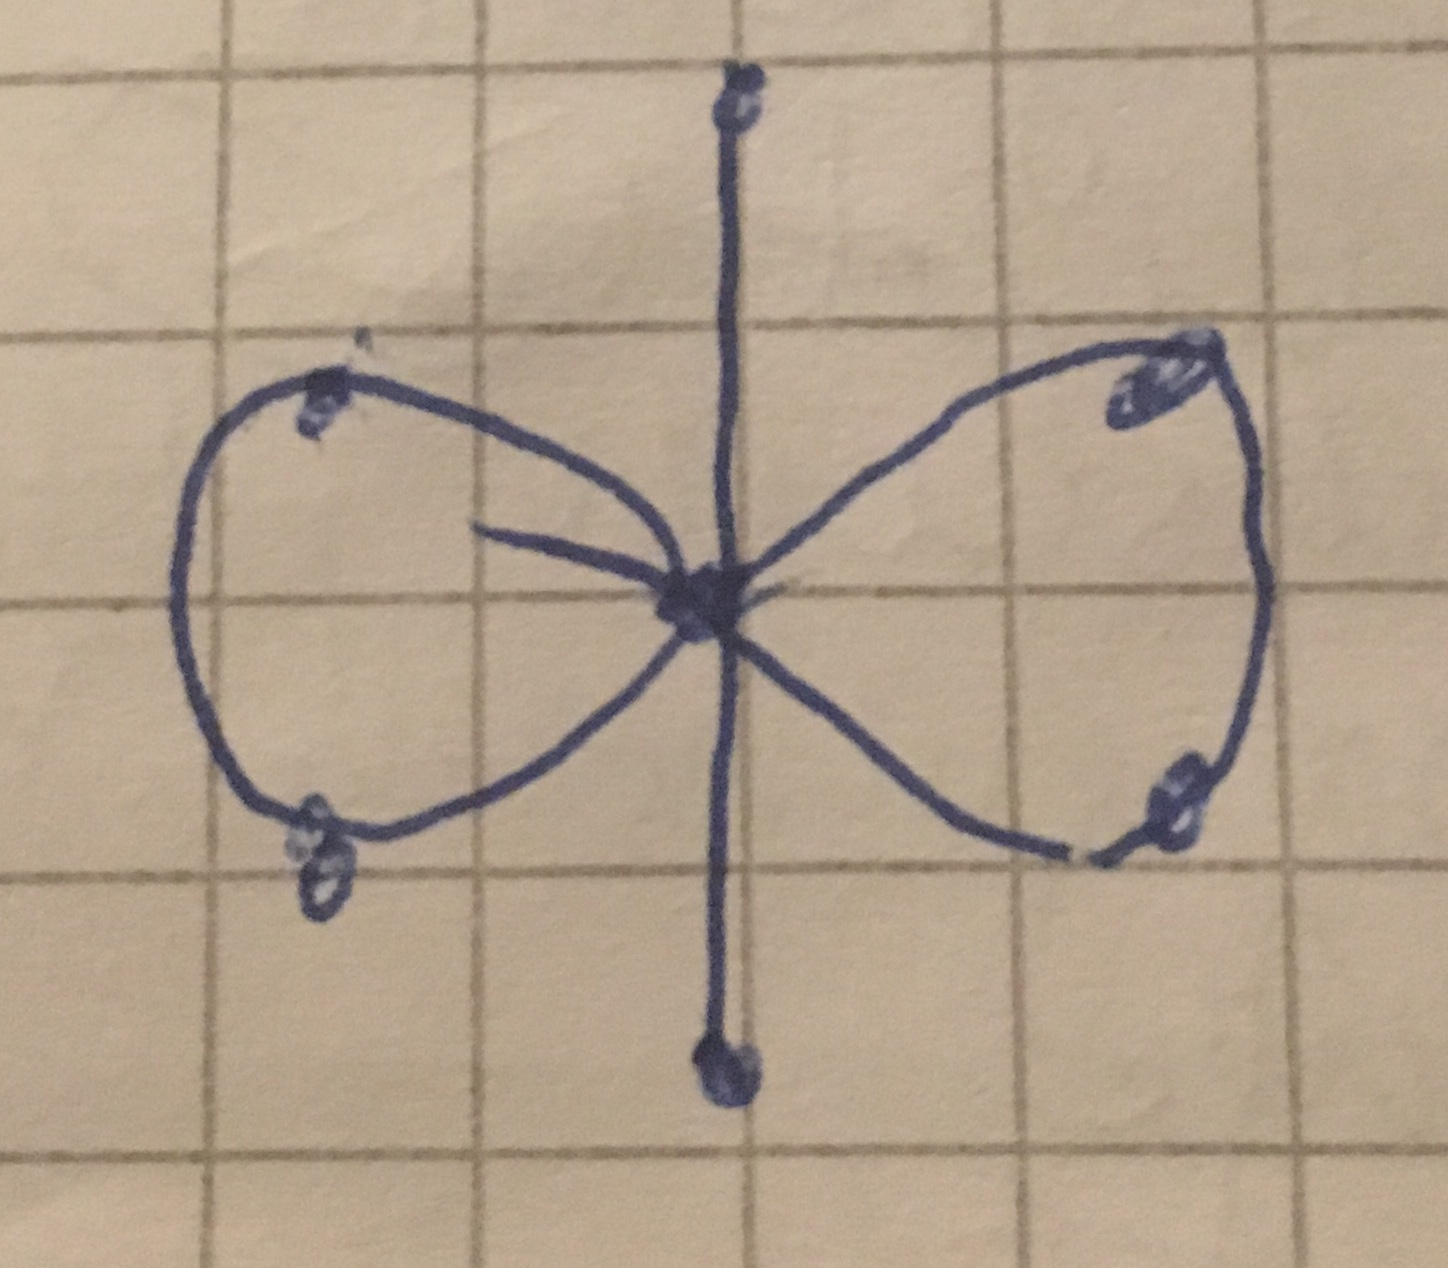
\includegraphics[width=0.3\textheight]{Abbildungen/Gesellschaft/Goettersymbol}
	\caption[Göttersymbol]{Das Symbol für die Götter}
	\label{fig:goettersymbol}
\end{figure}

\section{Geschichte}
Die hier erzählte Geschichte ist die vom Klerus verbreitete Sage über die Entstehung der Götter des Streits und der Heimtücke. \\\\
Es ist unklar, wie die Götter entstanden sind. 
Es geschah irgendwie irgendwann. 
Auf der noch recht unbewohnbaren Erde formten sie lebensfreundliches Gebiet mit ihrer jeweiligen Magie. 
Sie erschufen das Leben und ließen ihm seinen eigenen Lauf.\\
Nachdem sie jedoch viel Zeit damit verbracht hatten, sich an ihrem Paradies zu ergötzen, wollten sie auch Wesen nach ihrem Abbild schaffen und so lenkten sie das Leben und die Natur und brachten dadurch die Menschen hervor. 
Die Menschen, intelligent genug um Kultur aufzubringen, verfielen jedoch in viele Kriege. 
Mitgerissen aufgrund ihrer Ähnlichkeit und weil sie die Menschen so interessant fanden, integrierten sich die Götter in diese Streitigkeiten. 
Dabei nahmen sie die Positionen ihrer Menschengruppen an und halfen ihnen und wurden so langsam auch in einen Streit untereinander gezogen, wobei sie ihre negativen Seiten ausspielten.\\
Dies äußerte sich in vielen kleinen Dingen \textbf{(hier Geschichtchen einfügen)}, bis die Götter schließlich merkten, dass es so nicht weiter gehen kann. 
Sie setzten sich zusammen und kamen zum Schluss, dass sie, um wahre Leiter und Lenker des Lebens zu sein, ihre negativen Aspekte los werden müssten. 
Andernfalls würden ihre dunklen Seiten sie immer wieder übermannen können, was bereits große negative Folgen für alle Lebewesen hatte und auch wieder haben könnte.\\
Darum bereiteten die Götter ein Ritual vor, um perfekt zu werden und sich wortwörtlich von ihren schwachen Seiten rein zu waschen. 
Dazu begaben sie sich in einen See weitab der Zivilisation. 
Sie wuschen ihre schlechten Seiten von sich ab und versiegelten diese im See. 
\textbf{Allerdings gab es ein kleines Leck, durch welches kontinuierlich ein wenig von der Magie und dem Schlechten austrat.}\\
Danach treten die Götter lange Zeit nicht in Erscheinung. 
In der Nähe des Sees, den Bach hinunter, lebte ein Paar. 
All sein Trinkwasser nahm es aus dem Bach und all ihre Ernte wurde mit dem Wasser bewässert. 
So nahmen sie über Zeit immer mehr von dem Bösen in sich auf.
So wie ihre Macht und Magie wuchs, tat es auch das Böse in ihnen und verzehrte ihre guten Geister. 
Sie begannen aktiv das Böse aus der Umwelt und schließlich dem See zu absorbieren und wurden immer mächtiger und verdorbener. 
Sie führten Verwüstung und Zwist herbei und die Götter wurden auf sie aufmerksam. 
Ihre Versuche, sie zu bekämpfen und unter Kontrolle zu bekommen, scheiterten unter großen Verlusten in der Umwelt. 
Schließlich sahen die Götter ein, dass sie die beiden nicht besiegen konnten und unter all ihrer gebündelten Macht, um alle Lebewesen zu schütze, ersannen sie einen radikalen Plan.\\
Da die Götter zu verantworten hatten, dass diese Monster auf die Welt kamen, sahen sie es als ihre Pflicht, die Welt auch wieder von ihnen zu befreien. 
Aufgrund der zuvor genannten Umstände war die Maßnahme jedoch von drastischer Natur: sie hoben den Ort, auf dem sie die beiden bekämpften, aus der Erde heraus in den Himmel. 
Dort werden sie nun für alle Zeit gegen die beiden kämpfen und sie in Schach halten, damit das Leben auf der Erde geschützt ist.\\
Doch die beiden Bösen versuchen ihre Macht zu vergrößern, indem sie ihre Aktuelle auch dazu nutzen, den Lebewesen auf der Erde Böses einzuflüstern und sie zu manipulieren. 
\textbf{Die Erdenwesen sollen ihnen dienen.}\\
Bevor die guten Götter die Erdmasse mitsamt den Bösen in den Himmel aufgehoben haben, \textbf{erschufen sie gemeinsam einen Führer für die Toten}, der die verstorbenen Seelen zu ihnen bringen soll. 
Im Laufe der Zeit, in der sie ihre Pflichten als Götter und Führer der Welt etwas außen vor ließen, haben sie es geschafft, die Bösen zurück zu treiben. 
Nun gibt es nur noch Kampf auf einem kleinen Teil des Himmels-Brockens.\\
Nachdem die Toten verbrannt wurden, steigen ihre Seelen in den Himmel auf.
Wenn die Verstorbenen in ihrem Leben gut waren und sich nicht von den Einflüsterungen der bösen Götter haben verführen lassen, werden sie vom Seelenleiter hinüber geführt, auf dass sie mit ihrer Kraft die Götter unterstützen und in ihrem Paradies wohnen können. 
Die verdorbenen Seelen jedoch werden vom Seelenleiter zu Serro fehlgeleitet, damit sie nicht den Bösen helfen können, und auf dem Mond festhängen müssen.

\section{Götter}
In dem Land, in dem wir uns befinden, gibt es mehrere Götter. 
Regional unterscheidet sich die Wahl der bevorzugten Götter.
Diese sind Fiktion und existieren nicht wirklich; es gibt also auch keine Wunder, die von ihnen gewirkt werden. 
Allerdings interpretieren Menschen ja gerne sehr viel und sehen deshalb ein paar Dinge als Wunder an, die z.B. von den Priestern gemacht werden. 
Weil diese Priester gute Magier sind, aber das alles natürlich als Geschenk der Götter sehen.\\

Die Ausführungen im Folgenden stellen den Pantheon dar, wie er zur Zeit des Spiels angebetet wird.
Alle Namen sind vorläufig und mehr Möglichkeit gesehen, den Göttern und benannten Orten etwas mehr Griffigkeit zu geben.
Die Details, die im Folgenden gegeben werden (insbesondere die beispielhafte Mythen und Erzählungen über die Götter) dienen der Anschaulichkeit für uns und müssen sich nicht zwingend im Spiel wiederfinden.

\subsection{Asdir - Gott der Führung und des Schutzes}
Asdar ist der Anführer der Götter - nicht aufgrund außergewöhnlicher Stärke oder Charisma - Asdar ist nicht mächtiger als seine Mitgötter, sondern weil es seinem Wesen entspricht. 
Asdar ist standhaft, mutig und vertritt Führung durch Vorbild. 
Da, wo die Schutzbedürftigen verteidigt oder Verlorenen angeleitet werden müssen, ist Asdar in der ersten Reihe zu finden.
\begin{outline}
	\1 Aussehen 
		\2 großer Mann im mittleren Alter
		\2 kurze silberne Haare
		\2 häufig in Rüstung und mit alten Kampfnarben
	\1 Aspekte
		\2 Herrschaft und Führung
		\2 Kampf und Schutz
		\2 Vertreibung von Übel
	\1 Tugenden Asdars
		\2 Standhaftigkeit, Mut
		\2 körperliche Stärke und Macht
		\2 Opferbereitschaft
	\1 positive Gemüter: Mut, Macht, Kraft, Würde, Standhaftigkeit, Entscheidungsvermögen, Führungsqualitäten, Sicherheit, Intuition, Schutz
\end{outline}

\subsubsection{Weit bekannter Mythos Asdars}
Vor Urzeiten, als die Welt noch jünger war, streiften mächtige Monster durch die Lande und verbreiteten Angst und Schrecken. 
Es begab sich, dass Asdar, als einfacher Wanderer verkleidet, in einem Dorf Herberge suchte. 
Ein Lindwurm, eine mächtige Bestie mit einer geschuppten Haut härter als Stein und Klauen und Zähnen größer und schärfer als das beste Schwert der Menschen, fiel über das Dorf her, getrieben von unstillbarer Gier und Hunger. 
Und Asdar offenbarte sich in seiner Rüstung und sprach: 
``Wer bereit ist, sein Heim und seine Familie zu verteidigen, der nehme seine Waffe und kämpfe an meiner Seite.'' 
Und die Menschen folgten seinem Ruf, gewappnet mit jedweder Waffe die sie finden konnten. 
Der Kampf war lang und schwierig und manch einer wäre dem Hunger des Wurms zum Opfer gefallen, wenn Asdar die Angriffe nicht mit Schild und Rüstung abgefangen hätte. 
Doch mit seinem letzten Atemhauch gelang es dem Lindwurm noch, Klaue an Asdar zu legen und ihm eine weitere Narbe zu verpassen.




\subsection{Bouda - Göttin der Harmonie und des Wachstums}
Bouda ist die schaffende Gottheit des Pantheons. 
Nach ihrem Willen erwachsen neue Pflanzen in jedem Frühling, um den Hunger aller zu stillen. 
Nach ihrem Willen wird das Band der Ehe geformt, das zwei Menschen in Harmonie miteinander verbindet. 
Bouda akzeptiert alle als ihre Kinder und schenkt die Fähigkeit, zu vergeben und zu versöhnen.
\begin{outline}
	\1 Aussehen
		\2 ``Mutterfigur''
		\2 mittleres Alter 
		\2 kräftige Figur
		\2 alltägliche Kleidung 
	\1 Aspekte
		\2 Familie (Ehe und Elternschaft)
		\2 Ernte und Wachstum
		\2 Heilung
	\1 Tugenden Boudas
		\2 Gnade und Demut
		\2 Offenheit und Akzeptanz
		\2 nichterotische Liebe
	\1 positive Gemüter: Familie, Liebe, Selbstlosigkeit, Gnade, Mitgefühl, Vergebung, Demut, Reinheit, Frieden, Toleranz, Geborgenheit, Harmonie
\end{outline}

\subsubsection{Weit bekannter Mythos Boudas}
Vor Urzeiten, als die Welt noch jünger war, lagen die Reiche der Menschen beständig im Streit miteinander. 
Pakte wurden geschmiedet und gebrochen, ein Herrscher folgte auf den nächsten und keiner vermochte es, andauernden Frieden zu finden. 
Doch manchmal schmiedete das Schicksal seltsame Bande: 
es begab sich nämlich, dass die Thronfolger zweier verfeindeter Reiche in demselben Wald jagten und von einem Sturm von ihren jeweiligen Wegen abgebracht und in der Hütte einer alten Frau zusammengebracht wurden. 
Und als die beiden sich der Anziehung bewusst wurden, die zwischen ihnen zu erblühen begann, baten sie die alte Frau, ihre Vermählung vor Bouda zu bezeugen, auf dass selbst ihre Väter sie nicht mehr trennen könnten. 
Und die alte Frau schenkte ihnen zur Mitgift zwei Armreife, die das Band ihrer Vereinigung darstellen sollten. 
Und als die beiden Thronfolger heimkehrten, kam Friedfertigkeit über jeden, der die Reife der beiden sah. 
Und zum ersten Mal seit langem herrschte Frieden zwischen den Nationen.




\subsection{Rhena - Gott des Ausgleichs und der Gerechtigkeit}
Rhena lehrt die Menschen, die Bindungen zu ihren Mitmenschen ausgewogen zu halten. 
Sowohl Respektlosigkeit als auch übermäßige Ehrerbietung versäuern das Verhältnis zu den Mitmenschen und müssen daher vermieden werden. 
Dazu gehört, sich an die Gesetze und Regeln der Gesellschaft zu halten.
\begin{outline}
	\1 Aussehen 
		\2 alte Frau  -> "weise Frau"
		\2 hochgewachsen und hager
		\2 Gehstab/ Stecken
	\1 Aspekte
		\2 Gesetzgebung und Rechtsprechung
		\2 Handel
		\2 Weises Vorgehen \footnote{Leichte Überschneidung mit Faelans Aspekt}
	\1 Tugenden Rhenas
		\2 Disziplin und Respekt
		\2 stoisch und gelassen
		\2 streng mit sich selbst und Anderen
		\2 reich an Erfahrung
	\1 positive Gemüter: Höflichkeit, Disziplin, Gleichgewicht, Ruhe, Gelassenheit, Geduld, Wachstum, Ausgeglichenheit, Strenge, Heilung, Ausgleich, Urteilvermögen
\end{outline}

\subsubsection{Weit bekannter Mythos Rhenas}:
<Rhena fällt eine Richtspruch über ...>





\subsection{Erlin - Göttin der Lebensfreude und Liebe}
Erlin mag für manche wie der schwächste der Götter aussehen - seine Mythen berichten fast ausschließlich von Festen und Kunstwerken. 
Und dennoch ist Erlin einer der beliebtesten Götter im einfachen Volk. 
Jeder Reigen zum Mittsommerfest, jedes alkoholschwangere Fest und jeder stille (und jeder weniger stille) Moment der Zweisamkeit genießt Erlins Segen und Unterstützung.

Doch neben diesen ausgelassenen Momenten schenkt Erlin auch denen Lebensfreude und Hoffnung, die diese am dringensten benötigen. 
Diejenigen, die von Trauer oder Hoffnungslosigkeit niedergedrückt werden, hilft der Glaube an das Lebenswerte, um sich wieder aufzuraffen.
\begin{outline}
	\1 Aussehen 
		\2 junger Mann in Festtagskleidung
		\2 häufig zum Lachen aufgelegt
		\2 attraktiv 
	\1 Aspekte
		\2 erotische Liebe (als Vereinigung)
		\2 Feierlichkeiten
		\2 Kunst und Kultur
		\2 Trost und Hoffnung
	\1 Tugenden Erlins
		\2 Kreativität und Freigeistigkeit
		\2 zu Scherzen aufgelegt
		\2 charmant und fröhlich
	\1 positive Gemüter: Glück, Hingabe, Enthusiasmus, Fröhlichkeit, Freiheit, Menschlichkeit, Kunst, Kultur, Charme, Kreativität, Freude
\end{outline}

\subsubsection{Weit bekannter Mythos Erlins}
Vor Urzeiten, als die Welt noch jünger war, waren die Menschen eitel aufgrund ihrer eigenen Fertigkeiten. 
Glemric, Barde und Meister seiner Zunft, war einer dieser Menschen. 
Er rühmte sich seiner Künste mit Flöte und Harfe und behauptete, dass selbst Erlin selbst nicht mit ihm mithalten könne.
Und so kam es, dass eines Abends, als die Nächte kurz und der Mittsommer nahe war, eine junger Mann vor seiner Tür stand und ihn zu einem Wettbewerb herausforderte. 
Gäste wurden geladen, um die Kunstfertigkeit der Kontrahenten zu bewerten und sich ihrer Kunst zu erfreuen. 
Doch jedes Stück, das Glemric aufspielte, vermochte sein Gast zu überbieten, bis letzlich sogar Glemric selbst einsehen musste, dass er geschlagen war. 
Noch an diesem Abend gelobte er, seine Ehre wiederherzustellen und sich bei seinem Gast zu revanchieren. 
Und so geschah es, dass Glemric ein Jahr später in derselben Nacht Erlin zu einer Revanche herausforderte. 
Und die Geschichten erzählen, dass ihre Wettstreite sich bis heute in derselben Nacht fortsetzen.




\subsection{Faelan - Gott der Weisheit}
Weisheit kann viele Dinge bedeuten. 
Die Fähigkeit, Zusammenhänge zu begreifen und auszunutzen. 
Die Fähigkeit, den für sich selbst und Andere besten Weg zu erkennen. 
Und die Fähigkeit, aus dem Wenigen, was man hat, das Beste zu machen. 
Faelan verkörpert alle diese Aspekte. 
Einerseits ist er der Gott von Wissen und Gelehrsamkeit, der die Menschen Schrift, Wissen und Magie lehrt. 
Andererseits ist - beziehungsweise war - Faelan ein Gott der Schläue und der günstigen Gelegenheiten, der den Menschen überlegtes und zielstrebiges Handeln beibringt. 
Diese zweite Seite von Faelans Wesen ist mit dem Erstarken des Klerus immer mehr in Vergessenheit geraten, da die Verehrung eines Gottes der Diebe und Reisenden wenig erwünscht war.
\begin{outline}
	\1 Aussehen 
		\2 Junger Mann 
		\2 schlank und gelenkig
		\2 beständig neugierig
		\2 Wissen: trägt ein Buch und einen Kohlestift mit sich
		\2 Schläue: Tarnkappe oder ähnliches ``Werkzeug''
	\1 Aspekte
		\2 Weisheit und Verständnis
		\2 Schrift
		\2 Philosophie und andere Wissenschaften
		\2 Magie
	\1 Tugenden Faelans
		\2 Neugierig und wissbegierig
		\2 Lehrend
		\2 weise und beobachtend
	\1 positive Gemüter: Erleuchtung, Wissen, Verständnis, Konzentration, Wahrheit, Klarheit, (Um-)wandlung, Zielstrebigkeit, Weisheit, Aufstieg
\end{outline}
\subsubsection{Weit bekannter Mythos Faelans}
<Faelan stiehlt/vergibt einen Namen> 





\subsection{Der Flüsternde Schatten - Gott der Heimtücke}
Der Flüsternde Schatten -auch als ``Flüsterer'' bekannt - ist ein Gott, der aus einem Mangel an Emotionen entstanden ist.
Er ist manipulierend, rational und kühl. 
Mit einem wohlgesetzten Wispern schleicht er sich in die Köpfe der Menschen und lässt auch sie die Welt mit seinen Augen sehen. 
Und wer sich seines Flüsterns lange öffnet, der verliert Schritt für Schritt ebenso alle Fähigkeit zu eigenen Emotionen, bis der Mensch nicht viel mehr ist als ein lebender Schatten.
\begin{outline}
	\1 Aspekte
		\2 Feigheit
		\2 Gefühllosigkeit
		\2 Heimtücke
		\2 Rückgradlosigkeit
		\2 Eitelkeit
	\1 Plage
		\2 Depression und Trauer
		\2 grausames Kalkül
		\2 selbstsüchtige Hinterlist
		\2 Fanatismus
	\1 negative Gemüter: eingebildet, versteift, zwingend, ängstlich, heimtückisch, fanatisch, manipulativ, selbstüberschätzend, rücksichtslos, stolz, unterdrückend, hochnäsig,
	überheblich, arrogant, egoistisch, rückgratslos, feige, scheu, abhängig, Faul, gefühllos, eitel, misstrauisch, zynisch, nervös, voreilig, schadenfreudig
\end{outline}




\subsection{Drayl - Göttin des Streits}
Drayl ist eine Göttin, die aus einem Übermaß an Emotionen erwachsen ist. 
Jedes Übermaß an Emotionen führt Menschen zu Konflikten, bei denen nicht die gute Sache im Vordergrund steht, sondern die Menschen von Drayls Willen bessessen sind.
Drayl kann in vielerlei Formen erscheinen - sei es eine Axt, die einem Krieger ultimative Macht im Blutrausch verspricht, ein Schatz, der einen Händler zu gierigem Tun verleitet oder ein schönes Wesen, das zu hemmungsloser und aggressiver Wolllust verführt.

\begin{outline}
	\1 Aspekte
		\2 Wut
		\2 Neid
		\2 Gier
		\2 Chaos
	\1 Plage
		\2 Mania
		\2 Jähzorn
		\2 Instabilität
	\1 negative Gemüter: gierig,  habsüchtig,  streitsüchtig, störrisch, grausam, aggressiv, undiszipliniert, neidisch, unberechenbar, unaufmerksam, jähzornig, wollüstig, völlernd, 
	chaotisch, instabil, manisch
\end{outline}




\subsection{Das Göttersymbol} \label{sec:goettersymbol}
Beim Wasser-/Reinigungsritual, dem Abtrennungsritual oder einem anderen war die Aufstellung der fünf Götter und ihr Energiefluss wie dargestellt in Abb. \ref{fig:goetteraufstellung}. 
Denn die stärksten und direktesten Verbindundungen/Folgen ihrer Aspekte sind so. 
Das ergibt eine liegende acht, also das Symbol für Unendlichkeit --> 8 als heilige Zahl; 
Götter und ihre Macht sind unendlich.\\
\\
Mit den zwei Bösen Göttern: diese versuchen, alles zu spalten und zu zerstören. 
Das wird deutlich durch die Linie, welche die 8 versucht zu zerschneiden. 
Zudem zeigt es aber auch, wie durch die bösen Götter und zum Schutz des Lebens, ein Stück von der Erde abgetrennt werden musste. 
Des Weiteren mahnt es, wie unsere Schlechten Seiten immer Versuchung und Untergang sind — aber sie sind auch ein Teil von uns und wir müssen lernen, damit umzugehen und ihnen zu widerstehen. 
Aus diesen Aspekten ergibt sich das endgültige Göttersymbol wie dargestellt in Abb. \ref{fig:goettersymbol}.\\

\begin{figure}
	\centering
	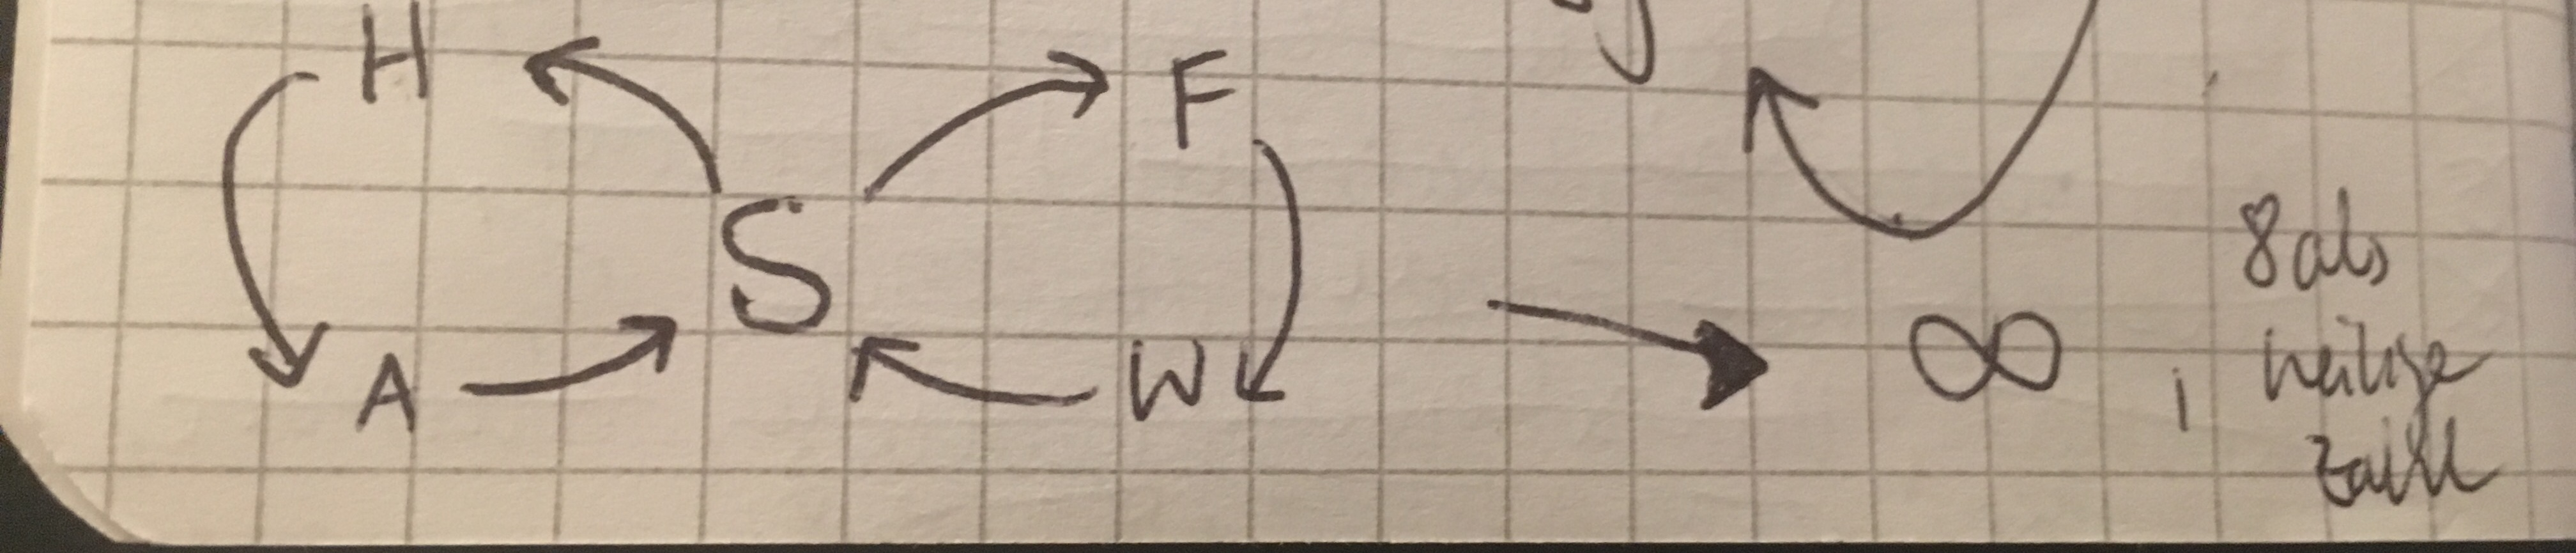
\includegraphics[width=0.7\linewidth]{Abbildungen/Gesellschaft/GoetteraufstellungbeiReinigungsritual}
	\caption{Aufstellung der Götter während des Reinigungsrituals}
	\label{fig:goetteraufstellung}
\end{figure}














\section{Klerus}\label{ch:klerus}
\textbf{Hier soll eine genauere Beschreibung des tatsächlichen Klerus erfolgen, also dem Teil der Struktur, der die Inhalte der Religion übermittelt. 
Zum Teil, der das Land verwaltet, siehe bitte \npref{ch:regierung}.} 

Da die Fähigkeit zur Nutzung der Magie natürlich auch von den Göttern kommt (nur wenige Arten können dies, ein paar Pflanzen, ein paar Tiere und darunter die menschlichen Arten (und unbekannterweise natürlich auch Mikroorganismen)), ist die Intensität, in der man Magie nutzen kann, natürlich auch ein Zeichen für die Gunst der Götter. 
Demnach müssen außerordentlich Begabte stark in der Gunst stehen und daher auch ihr Leben den Göttern widmen - aka in den Orden gehen. 
Tatsächlich ist das aber auch ein Mittel des Ordens, diese mächtigen Leute zu kontrollieren, da sie die nach ihrer Art prägen und unter ihrer Anweisung haben

\subsection{Stände der Gesellschaft}\label{ch:staende}
In der Gesellschaft unserer Nation gibt es vier gesellschaftliche Stände, die sich jeweils durch Privilegien und Status unterscheiden. 
Diese Hierarchie ist teilweise durch die Religion und Regierungsstruktur motiviert, allerdings nicht wirklich im Gesetz kodifiziert. Es mag zwar keine gesetzlichen Strafen geben, 
wenn bsp ein Bürger einem Geistlichen widerspricht; es ist aber trotzdem ungern gesehen und kann leicht zu unangenehmen Konsequenzen führen.
\begin{outline}
	\1 \emph{Göttersprecher} ( $=$ Geistliche)
		\2 alle Magier des Ordens sind in diesem Stand
		\2 Reichtum und Einfluss sind relativ hoch 
	\1 \emph{Gesegnete}
		\2 Person mit außergewöhnlichen Fähigkeiten auf einem bestimmten Gebiet
		\2 Vom Klerus ausgebildet/ angeworben
		\2 häufig wohlhabend, mit Einfluss
		\2 Bsp: hochrangige Militärs, Bürokraten, Schöffen,  ... (Spione)
	\1 \emph{Freie Bürger}
		\2 Landloser Bewohner (v.A. in größeren Gemeinden und Städten)
		\2 lebt nicht zwingend von Landwirtschaft, sondern von Handel/Handwerk
		\2 häufig etwas wohlhabender als die Leibeigenen
		\2 reiche Bauern können in diesen Stand aufsteigen
	\1 \emph{Leibeigene}
		\2 Großteil der Bevölkerung
		\2 an das Land gebunden, auf dem sie leben (Beruf, Wohnort nicht frei wählbar)
		\2 unter der Obhut eines Verwalter, dem sie abgaben-pflichtig sind
		\2 arm und von der Kirche mit dem nötigsten versorgt
\end{outline}

\emph{Magieadel}: Aufgrund der Vererbbarkeit von magischen Fähigkeiten (und Intensität) ist es sehr wahrscheinlich, dass die Kinder von Göttersprechern erneut Göttersprecher werden. 
Dadurch ist es Familien mit außergewöhnlichen Fähigkeiten möglich, über mehrere Generationen Reichtum und Beziehungen anzuhäufen. 
Zudem wird es für diese einfacher möglich, begabten Kindern ihren Posten zu vererben.



\subsection{Aufbau \& Struktur}
Den verschiedenen Rängen des Klerus haben neben religiösen Pflichten - Predigten, Durchführung von Riten und Anleitung der Gläubigen - auch organisatorische Pflichten auszuführen. 
In ihrem Zuständigkeitsbereich stellt der jeweilige Göttersprecher die höchste Regierungsauthorität dar. 
Alle Verwaltungsentscheidungen werden (mittelbar) durch ihn getroffen.
Dabei werden die meisten Göttersprecher von einer Reihe untergebener Gesegneter - zumeist ausgebildete Bürokraten - unterstützt.

Die meisten Göttersprecher (mit Ausnahmen) verschreiben sich dem Dienst an allen fünf Göttern, können aber Favoriten haben. 
\footnote{Sollte es Tempelanlagen und Priester zu einer Gottheit geben?}
Zudem sind viele (v.A. in den unteren Rängen) ernsthaft daran interessiert, ihren Schutzbefohlenen Gutes zu tun und nicht auf persönliche Bereicherung aus.

Der Klerus teilt sich grob auf drei verschiedene Ränge auf, die jeweils den übergeordneten Rängen gehorchen müssen. 
Alle diese Ämter sind (abgesehen von Beförderungen) auf Lebenszeit.
Das Geschlecht hat keinen Einfluss auf die Zulässigkeit für bestimmte Würden.
\footnote{Der Einfachheit halber wird das männliche Wort verwendet.}
\begin{outline}
	\1 \emph{Prediger}
		\2 zuständig für eine Gemeinde
		\footnote{Das können ein oder zwei Dörfer sein. In größeren Städten existieren teilweise sogar mehrere Gemeinden}
		\2 sammelt Abgaben an die Kirche ein, kontrolliert Versorgung von der Kirche (Heilmittel, ...)
		\2 hält Dorfgerichte, Predigten, Schule/religiöse Erziehung
		\footnote{Leibeigene erlernen rudimentär Lesen/Schreiben/Rechnen und werden in Religion und Geschichte belehrt}
	\1 \emph{Bischof}
		\2 zuständig für eine Region
		\footnote{Regieren häufig von der größten Stadt der Region aus.}
		\2 halten selten/nie Predigten (da keine eigene Gemeinde)
		\2 Kontrolle von Ressourcen der Kirche \& höchste religiöse Authorität der Region
	\1 \emph{Der Rat der Fünf}
		\2 effektives Regierungsorgan der Nation 
		\2 vier Bischöfe + Abt(siehe unten), die sich jeweils dem Dienst an einem der fünf Götter verschworen haben -> "Erster Diener / Erste Dienerin ..."
		\2 kommen aus Gebieten, wo die Verehrung der jeweiligen Gottheit am stärksten ist (Diener Asdirs aus der Hauptstadt)
		\2 haben Kontrolle über ein Viertel der Nation (und alle enthaltenen Bistümer)
		\2 Authorität über Riten und Dogmen ihrer jeweiligen Gottheit
		\2 bei Wahl eines neuen Ersten Dieners: Bischöfe der jew. Region wählen unter sich
		\2 Erster Diener ernennt neue Bischöfe der jew. Region (nach Ableben des alten Bischofs)
\end{outline}
\emph{Klöster} sind Stätten des Wissens und der Forschung. Hier wird neben Geschichte, Philosophie, Theologie/Theosophie auch an Magie geforscht. 
Die meisten Klöster beschränken sich allerdings auf eine Form von Magie und bilden in dieser Form auch aus.\\
Jedes Kloster wird von einem Abt geleitet, der vom Rang her einem Bischof entspricht. 
Da die meisten Klöster sich Faelan verschreiben, ist der Erste Diener Faelans immer ein Abt. 
Ihm untersteht der Geheimdienst und die Archive des Ordens.

\subsection{Riten}
\paragraph{Ideen}
\begin{outline}
	\1 Predigt --> worshipping mit Gesang
\end{outline}




\subsubsection{Tod}
Wenn jemand stirbt, so muss er verbrannt werden, damit seine Seele vom Körper frei wird und in den Himmel zu den Göttern aufsteigen kann und ihnen im Kampf gegen die bösen Götter beistehen kann. 
Das sollte optimal dann erfolgen, wenn die zweite Erde am Himmel steht, damit er schnell dort hingelangt. 
Gotteslästerer und böse Leute werden nicht verbrannt, sondern begraben. 
So können sie den Bösen Göttern nicht beistehen.
Demnach ist es sehr schlimm, wenn jemand nach seinem Tod nicht angemessen aufbereitet und vor allem verbrannt wird!

\subsection{Gebäude}
